\documentclass[a4paper, 12pt,oneside]{article}
\usepackage{graphicx} % Required for inserting images
\usepackage[top=2.5cm, bottom=2cm, left=2cm, right=2cm]{geometry}
\usepackage[french]{babel}  % Définit le français comme langue principale
\usepackage[utf8]{inputenc}  % Gère les accents et caractères spéciaux (si nécessaire)
\usepackage[T1]{fontenc}
\usepackage[colorlinks,bookmarks=false,linkcolor=black,urlcolor=blue, citecolor=black]{hyperref}
\usepackage{units}
\usepackage{verbatim}
\usepackage{verbdef}% http://ctan.org/pkg/verbdef
\usepackage{amsmath}
\usepackage{amssymb}
\usepackage{wrapfig}
\usepackage{subcaption}
\usepackage{caption}
\usepackage{float}
\usepackage[export]{adjustbox}
\usepackage{upgreek}
\usepackage{hyperref}
%Pour changer la taille des titres de section et subsection. Ajoutez manuellement les autres styles si besoin.
\makeatletter
\renewcommand{\section}{\@startsection {section}{1}{\z@}%
             {-3.5ex \@plus -1ex \@minus -.2ex}%
             {2.3ex \@plus.2ex}%
             {\normalfont\normalsize\bfseries}}
\makeatother

\makeatletter
\renewcommand{\subsection}{\@startsection {subsection}{1}{\z@}%
             {-3.5ex \@plus -1ex \@minus -.2ex}%
             {2.3ex \@plus.2ex}%
             {\normalfont\normalsize\bfseries}}
\makeatother

\graphicspath{{Graphes/}}

\begin{document}
\title{\normalsize{Lab Work Report - Group N$^\circ$\\ XX - Experiment}}
\date{\normalsize{\today}}
\author{\normalsize{Name} 1\and \normalsize{Name 2}}

\begin{center}
\large\textbf{\sffamily Expérience N$^\circ$F7. Interférométrie}\\%
\large\sffamily Groupe N$^\circ$22: Armand Le Douarec, Maxime Chatelin\\%
\large\sffamily\today\quad   Assistant -  Emiliano Cruz Aranda \\%
\end{center}

\section{Introduction}

L'interférométrie, technique au cœur de nombreuses avancées scientifiques récentes, s'est imposée comme un outil essentiel en physique pour sonder des phénomènes d'une précision inégalée. En exploitant les interférences des ondes, cette méthode offre une précision exceptionnelle, révélant des détails autrement invisibles. L'interféromètre de Michelson [\ref{ref1}], emblème de cette technique, a marqué la physique dès la fin du XIXe siècle avec l'expérience de Michelson-Morley [\ref{ref2}], réfutant la théorie de l'éther. Cet outil est aujourd'hui utilisé dans des projets de pointe, comme la détection des ondes gravitationnelles avec LIGO [\ref{ref3}] et Virgo [\ref{ref4}]. Dans ce rapport, cet instrument est utilisé pour déterminer la longueur d'onde d'un laser monochromatique, mesurer le coefficient de dilatation thermique de différents métaux, étudier la magnétostriction, et calculer l'indice de réfraction de l'air, montrant ainsi sa polyvalence et son extrême précision.

\section{Théorie}

La lumière, comme toutes les ondes électromagnétiques, possède un comportement ondulatoire. Pour deux ondes synchrones et cohérentes qui interfèrent, l’amplitude résultante dépend de la différence de phase entre elles : une superposition en phase créé une interférence constructive, doublant ainsi l’amplitude, tandis qu’un déphasage complet conduit à une interférence destructive, amenant à la nullité de l'amplitude. Cette étude des interférences particulièrement utile correspond à la caractéristique principale de l'interféromètre dans le cadre de ces expériences [\ref{ref5}].

\paragraph{Interféromètre de Michelson}

\begin{wrapfigure}{h}{0.4\textwidth}
    \centering
    \includegraphics[width=1\linewidth]{Schémas/Montage_Michelson.jpg}
    \captionsetup{justification=centering}
    \caption{Interféromètre de Michelson.}
    \label{fig1}
\end{wrapfigure}


L’interféromètre de Michelson visible sur la Fig.(\ref{fig1}) repose précisément sur ce principe d’interférence. Un faisceau de lumière est divisé, suit deux chemins différents, puis est recombiné pour créer des interférences exploitables. Le faisceau atteint le diviseur de faisceau BS qui le sépare en deux ondes : une onde transmise I$_t$ dirigée vers le miroir fixe M1 et une onde réfléchie I$_r$ envoyée vers un miroir mobile M2.
Les faisceaux effectuent des trajets différents étant réfléchis par M1 ou M2, puis recombinés sur le diviseur de faisceau [\ref{ref5}]. La différence de distance parcourue par les rayons, liée aux chemins optiques entre les miroirs, provoque un déphasage, créant ainsi des interférences observables sur un écran via le miroir M3. En ajustant la position du miroir M2, la différence de chemin optique $\Delta L$ est modifiée, entraînant alors un défilement des franges d’interférence sur l’écran.
Le nombre de franges observées $N$, correspondant à la variation du chemin optique, est directement lié à la longueur d’onde $\lambda_0$ du laser par la relation [\ref{ref5}] :

\begin{equation}
    \Delta L=\frac{N\lambda_0}{2}.
\label{eq1}
\end{equation}

Cette relation permet de mesurer expérimentalement $\lambda_0$, en calculant le déplacement du miroir $\Delta L$ et le nombre de franges observées $N$.

\paragraph{Dilatation thermique}

\begin{wrapfigure}{h}{0.4\textwidth}
    \centering
    \includegraphics[width=1\linewidth]{Schémas/Dilatation_Thermique.jpg}
    \captionsetup{justification=centering}
    \caption{Interféromètre de Michelson pour l'étude de la dilatation thermique.}
    \label{fig2}
\end{wrapfigure}

L’interféromètre de Michelson est aussi employé pour étudier des propriétés thermiques des matériaux, telle que la dilatation thermique. Cette dernière repose sur l'élongation d'un solide avec la température, selon une loi proportionnelle [\ref{ref5}]: 

\begin{equation}
   l_T = l_0(1+\alpha T) 
\label{eq2}
\end{equation}

\noindent avec $l_0$ la longueur de l’échantillon à température ambiante, $l_T$ la longueur de l’échantillon à température $T$. Le coefficient de dilatation thermique linéaire $\alpha$ est défini comme la variation relative de longueur d’un solide pour une augmentation de température d’un degré Celsius, et $T$ est la température du matériau en degrés Celsius.

Un échantillon métallique chauffé, voit sa longueur modifié, qui induit à son tour une variation du trajet optique parcouru par le faisceau lumineux. La dilatation du métal est observée à travers le défilement des franges d’interférence sur l’écran. Ce défilement est lié au changement de longueur $\Delta L$ par la relation [\ref{ref5}]:
\begin{equation}
    \Delta L = l_0 \cdot \alpha \cdot \Delta T
\label{eq3}
\end{equation}

\noindent avec $\Delta T$ la variation de température en degré Celsius. En mesurant le nombre de franges $N$ qui défilent lors de la dilatation et connaissant la longueur d’onde $\lambda_0$ du laser, la relation suivante utilisant l'Eq.(\ref{eq1}) et l'Eq.(\ref{eq3}) permet de relier $N$ à $\alpha$ et obtenir la relation [\ref{ref5}] :
\begin{equation}
    N = \frac{2 l_0 \alpha \Delta T}{\lambda_0}
\label{eq4}
\end{equation}

\paragraph{Magnétostriction}

La magnétostriction est un phénomène par lequel certains matériaux ferromagnétiques subissent une déformation lorsqu'ils sont soumis à un champ magnétique externe. Cette variation de longueur relative $\Delta L/ L$, avec $L$ la longueur initiale du matériau et $\Delta L$ donné par l’Eq.(\ref{eq1}), est une conséquence directe du réarrangement des domaines magnétiques internes du matériau sous l'influence d'un champ magnétique $B$. Le champ magnétique est appliqué à l’aide d’un solénoïde entourant l’échantillon, et son intensité est donnée par l’équation [\ref{ref5}] :
\begin{equation}
    B = \frac{\mu_0 N_s I}{l_s}
\label{eq5}
\end{equation}

\noindent où $\mu_0=1.256 \cdot 10^{-6}$\,kg·m·A$^{-2}$·s$^{-2}$ [\ref{ref6}] est la perméabilité du vide, $N_s$ est le nombre de tours du solénoïde, $I$ l’intensité du courant qui le traverse, et $l_s$ la longueur du solénoïde.

\paragraph{Indice de réfraction de l'air}

Pour mesurer l'indice de réfraction de l'air, un dispositif expérimental est utilisé, il contient une enceinte de longueur $l$ placée sur le chemin optique du rayon lumineux avant d'atteindre le miroir M1. Lorsque l'enceinte est remplie d'un gaz d'indice de réfraction $n$, la lumière ralentit, entraînant un déphasage donné par [\ref{ref5}] :

\begin{equation}
    \Delta L = 2l(n - 1)
\label{eq6}
\end{equation}

En substituant $\Delta L$ dans l'équation précédente (Eq.(\ref{eq6})) et en dérivant par rapport à la pression $p$, la relation suivante est trouvée [\ref{ref5}] :

\begin{equation}
    \frac{dN}{dp} = \frac{2l}{\lambda_0} \frac{dn}{dp}
\label{eq7}
\end{equation}

Pour un gaz parfait, l'indice de réfraction peut être exprimé comme suit [\ref{ref5}] :

\begin{equation}
    n - 1 = (n_0 - 1)\frac{p T_0}{p_0 T}
\label{eq8}
\end{equation}

où $n_0$ est l'indice de réfraction de l'air, $T$ la température ambiante, $T_0 = 273 \,$K, et $p_0 = 101325 \,$ Pa [\ref{ref5}]. En remplaçant cette expression dans l’Eq.(\ref{eq8}) est obtenue l'équation suivante [\ref{ref5}] :

\begin{equation}
    n_0 - 1 = \frac{dN}{dp} \frac{\lambda_0 p_0 T}{2l T_0}
\label{eq9}
\end{equation}

Ainsi, pour déterminer l'indice de réfraction de l'air, l'enceinte est remplie d'air à différentes pressions, de l'ordre de $10^4$\,Pa. Pour chaque pression, l’enceinte est vidée par microfuite et le nombre de franges $N = N(p)$ qui défilent à l'écran sont comptées.


\section{Démarche expérimentale}

Le montage utilisé est composé d'un laser He-Ne de 2\,mW, de deux lentilles convergentes L1 et L2, de distance focale $f_1 = (5.0\,\pm\,0.1)\,$mm et $f_2=(50.0\,\pm\,0.1)\,$mm, de deux miroirs M1 et M2 ainsi que d'un diviseur de rayons BS.

\paragraph{Longueur d'onde $\lambda_0$}
La première expérience permet de déterminer la longueur d'onde du laser utilisée. Sa mesure est directement effectuée en variant la longueur $\Delta L$ à l'aide d'une vis micrométrique jusqu'à voir $(100\,\pm\,10)$ franges défilées sur l'écran et en utilisant l'Eq.(\ref{eq1}).

\paragraph{Coefficient de dilatation thermique}

Une fois ces grandeurs connues, il est possible de déterminer de nouvelles grandeurs telles que les coefficients de dilatation thermique du cuivre et de l'aluminium. Pour chaque expérience la batônnet du matériau utilisé est de longueur $L = (11.00\,\pm\,0.05)\,$cm. Pour augmenter la température de l'objet, un générateur de tension est d'usage, avec une tension $U=(0.5\,\pm\,0.1)\,$V,  et une intensité choisie à $I=(3.0\,\pm\,0.1)\,$A. La température est relevée à l'aide d'un thermocouple. Les coefficients sont trouvés à partir de l'Eq.(\ref{eq4}).

\paragraph{Magnétostriction}

L'interféromètre de Michelson permet de mesurer l'élongation de matériaux ferromagnétiques soumis à un champ magnétique $B$. À l'aide d'une solénoïde entourant l’échantillon, le champ créé est dirigé le long de son axe. L'intensité résultante est donnée par l'Eq.(\ref{eq5}). Pour un nombre de spires de 1000 et la longueur de la bobine $l_s = (6.2\,\pm\,0.1)\,$cm. L'intensité varie entre $(0.0\pm0.1)$\, A et $(2.0\pm0.1)$\,A.

\paragraph{Indice de réfraction de l'air}
Pour cette dernière expérience, une enceinte de longueur $l=(6\,\pm\,1)\,$cm, depuis laquelle l'air est pompée, est utilisée. Cette enceinte est placée entre le BS et M1 sur la Fig.(\ref{fig1}). La pression ambiante est de $p_0=(968\,\pm\,1)\,$mbar et la température ambiante est $T=(22.0\,\pm\,0.1)\,^\circ$C. La pression $p$ dans cette enceinte est varie de $(30\,\pm\,5)\,$kPa à  $(70\,\pm\,5)\,$kPa par pas de 10\,kPa. Enfin, à partir de l'Eq.(\ref{eq9}), des grandeurs connues et du coefficient $\text{d}N/\text{d}p$ calculé sur le graphe, l'indice de réfraction de l'air est déduit.

\section{Résultats}

Plusieurs tests préliminaires ont révélé la sensibilité de l’interféromètre. Une pression sur le plateau ou de l'air soufflé sur le chemin du laser ont provoqué un défilement rapide de nombreuses franges à l'écran.

\paragraph{Longueur d'onde $\lambda _0$}

L'expérience afin de déterminer la longueur d'onde $\lambda _0$ du laser consiste à mesurer le déplacement $\Delta L$ du miroir M1 pour un défilement à l'écran de 100 franges. Plusieurs mesures ont été réalisées, sont indiquées dans le Tab.(\ref{tab1}) et sont comparées à la valeur de référence $\lambda _{0,\,\text{th}}$ de 632.8\,nm [\ref{ref7}]. Par ailleurs, pour le reste des expériences, la valeur utilisée pour la longueur d'onde du laser est la valeur de référence $\lambda _{0,\,\text{th}}$.

\begin{table}[H]
    \centering
    \begin{minipage}{0.35\textwidth}  % Ajustez la largeur du tableau
        \centering
        \begin{tabular}{|c||c|c|}
        \hline
        & Mesure 1 & Mesure 2\\
        \hline
        $\Delta L\,$[$\mathrm{\mu}m$] & $40\,\pm\,1$ & $37\,\pm\,1$  \\
        \hline
        $\lambda_{0,\,\text{exp}}\,$[nm]  & $800\,\pm\,90$ & $740\,\pm\,90$\\
        \hline
        $\epsilon\,$[\%] & 26 & 17\\
        \hline
        \end{tabular}
    \end{minipage}%
    \hfill
    \begin{minipage}{0.6\textwidth}  % Ajustez la largeur de la légende
        \captionsetup{justification=centering}  % Légende alignée à gauche
        \caption{Valeurs de la longueur d’onde du laser mesurée expérimentalement $\lambda_{0,\,\text{exp}}$ et erreur relative $\epsilon$ par rapport à la valeur théorique $\lambda_{0,\,\text{th}} = 632.8\,$nm [\ref{ref7}] à l'aide de l'élongation $\Delta L$ du matériau pour voir $N=100$ franges défilées sur l'écran.}
        \label{tab1}
    \end{minipage}
\end{table}

\paragraph{Coefficient de dilatation thermique}

La Fig.(\ref{fig3}) présente un graphe du nombre de franges défilées par rapport à l'augmentation de la température. Une régression linéaire est effectuée et permet, avec l'utilisation de l'Eq.(\ref{eq4}), d'en déduire $\alpha_{\text{exp}}$ pour le cuivre et pour l'aluminium. Les valeurs trouvées sont indiquées dans le Tab.(\ref{tab2}) et comparées aux valeurs tabulées $\alpha _{\text{th}}$ [\ref{ref8}]

\begin{figure}[h]
    \centering
    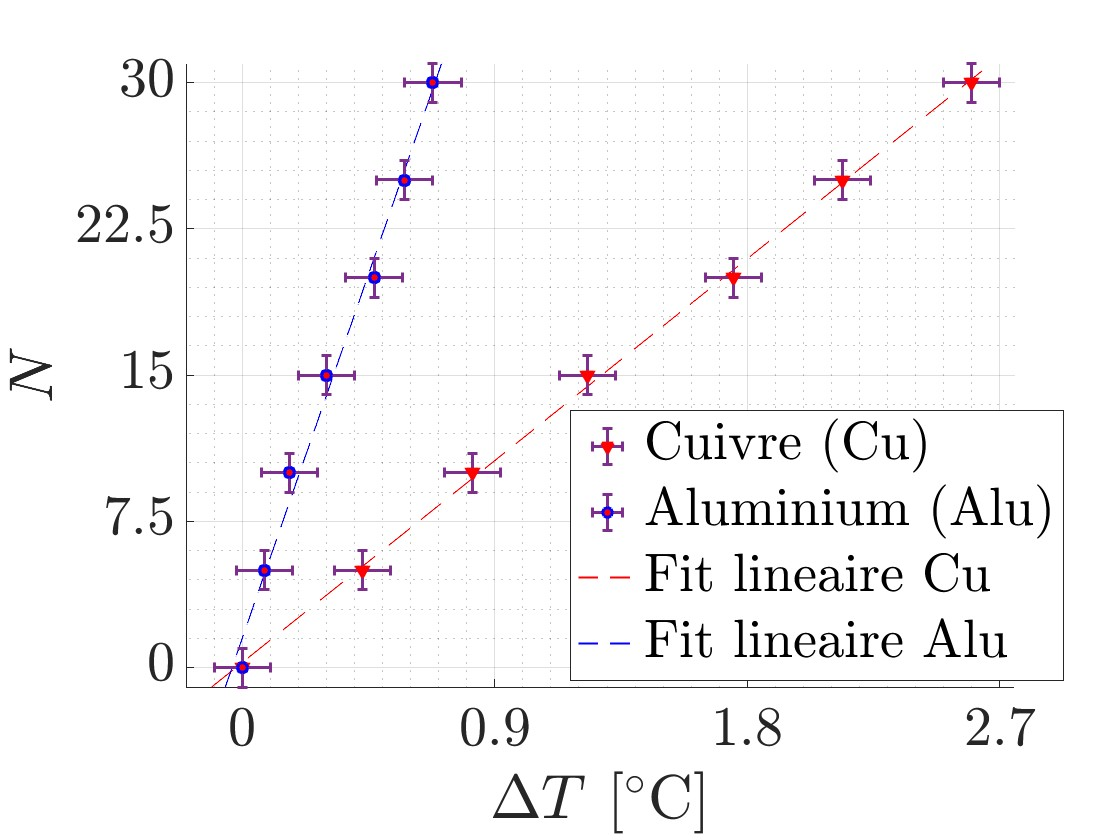
\includegraphics[width=0.45\textwidth]{Graphes/franges_mat.jpg}
    \captionsetup{justification=centering}
    \caption{Graphe mettant en relation l'augmentation de la température $\Delta T$[°C] du barreau de cuivre ou d'aluminium et le nombre de franges défilant $N$}
    \label{fig3}
\end{figure}

\begin{table}[h]
    \centering
    \begin{tabular}{|c||c|c|}
        \hline
        Matériau & Cuivre & Aluminium\\
        \hline        $\alpha_{\text{exp}}[^\circ\text{C}^{-1}$] & $(33\,\pm\,1)\cdot10^{-6}$ & $(120\,\pm\,50)\cdot10^{-6}$  \\
        \hline        $\alpha_{\text{th}}[^\circ\text{C}^{-1}$]  & $17\cdot10^{-6}$ & $26\cdot10^{-6}$\\
        \hline
        $\epsilon\,$[\%] & 94 & 362\\
        \hline
    \end{tabular}
    \captionsetup{justification=centering}
    \caption{Valeurs des coefficients de dilatation thermique obtenus expérimentalement $\alpha_{\text{exp}}$ et erreurs relatives $\epsilon$ par rapport aux valeurs théoriques $\alpha_{\text{th}}$ [\ref{ref8}]}
    \label{tab2}
\end{table}
\vspace{-0.2cm}
\paragraph{Magnétostriction}
Cette partie consiste à étudier la magnétostriction d’un barreau d’acier soumis à un champ magnétique $B$. C'est pourquoi la Fig.(\ref{fig4}) propose l’allongement relatif $\Delta L/L$ en fonction de la norme du champ magnétique appliqué. Étant donné un défilement plus rapide des franges avec l'augmentation de $B$, l'erreur de l'allongement relatif du barreau augmente à son tour (visible via les barres d'erreur sur la Fig.(\ref{fig4})).

\begin{figure}[H]
    \centering
    \begin{minipage}{0.45\textwidth}
        \centering
        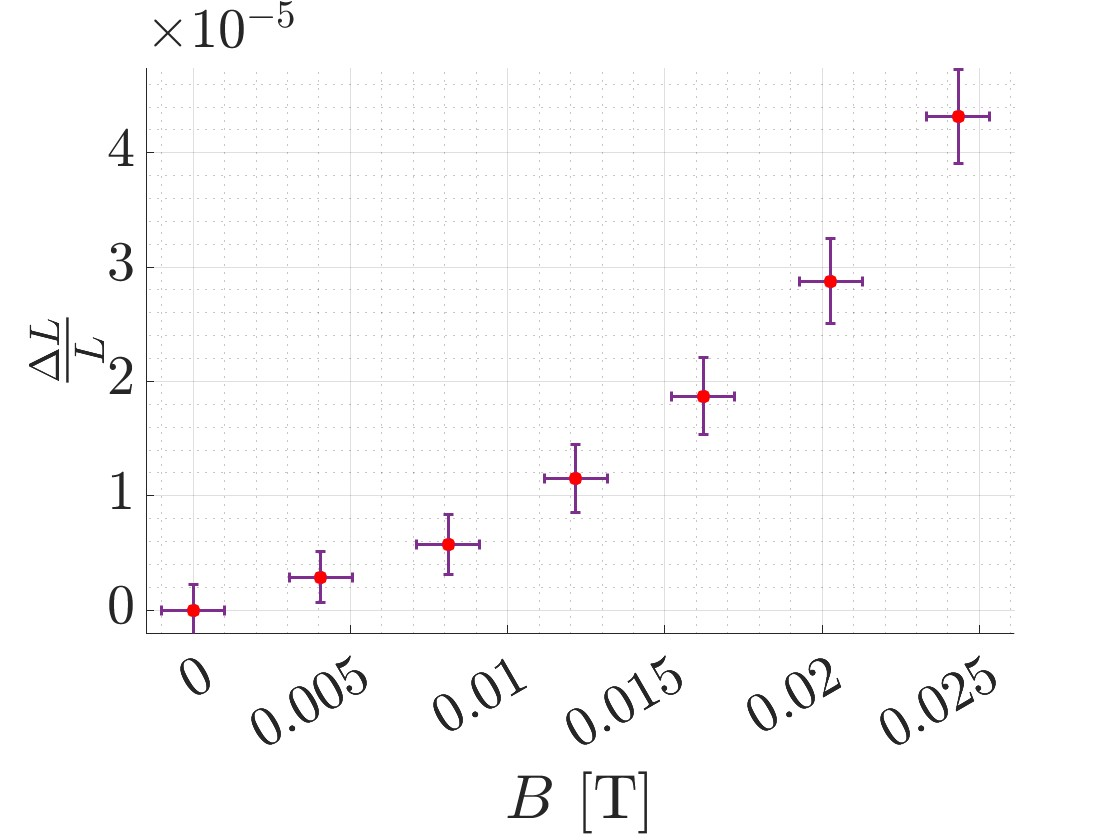
\includegraphics[width=\linewidth]{Graphes/franges_mag.jpg}
        \captionsetup{justification=centering}
        \caption{Variation de la longueur relative $\Delta L/L$ du barreau d'acier en fonction du champ magnétique $B$.}
        \label{fig4}
    \end{minipage}
    \hfill
    \begin{minipage}{0.45\textwidth}
        \centering
        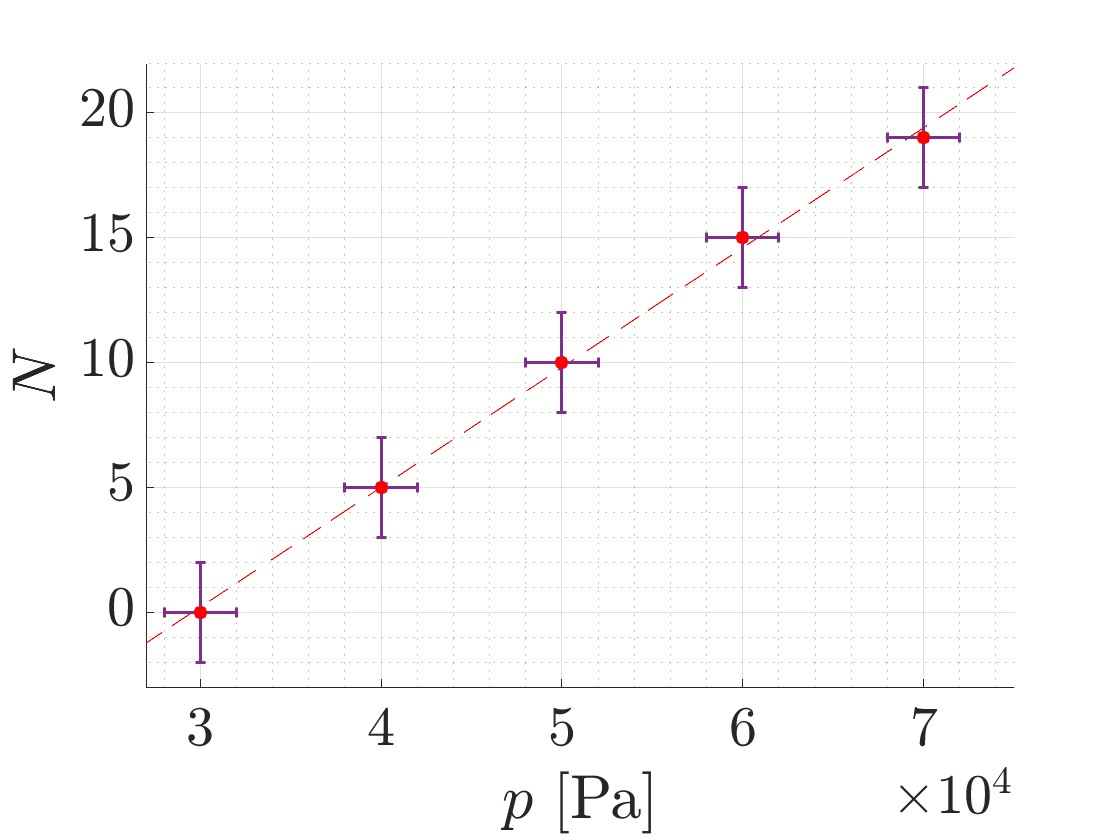
\includegraphics[width=\linewidth]{Graphes/franges_pression.jpg}
        \captionsetup{justification=centering}
        \caption{Nombre $N$ de franges qui défilent en fonction de la pression $p$ dans la chambre à air.}
        \label{fig5}
    \end{minipage}
\end{figure}
\vspace{-0.8cm}
\paragraph{Indice de réfraction de l'air}

La Fig.(\ref{fig5}) montre la variation du nombre de franges défilées $N$ en fonction de la pression $p$. La pente obtenue, à l'aide d'un fit linéaire est d$N/$d$p=(4.8\pm0.4) \cdot 10^{-4}$\,Pa$^{-1}$, pour un intervalle de confiance de 95\,\%. À l'aide de l'Eq.(\ref{eq9}), il est possible de calculer $(n_0 - 1) = (2.7 \,\pm\, 0.5) \cdot 10^{-4}$\,Pa. Comparée à la valeur tabulée à 22°C de $(n_{0,th} - 1) = 2.69 \cdot 10^{-4}$\,Pa  [\ref{ref9}], l'erreur relative est de 0.4\,\%.
\vspace{-0.3cm}
\section{Discussion}
\vspace{-0.3cm}
La première approche, essentielle, est de relever la sensibilité de l'interféromètre. Au moindre faux geste, appui sur la table ou souffle sur le trajet du laser, l'expérience prend une toute autre tournure, l'appareil est sensible aux légères perturbations. Le montage de l'appareil requiert une immense précision, qui, lorsqu'elle n'est pas  atteinte, peut rendre les résultats difficiles à correctement mesurer. Ceci rend l'appareil complexe à utiliser et constitue source d'erreurs significatives dans ce TP.

\paragraph{Longueur d'onde $\lambda _0$}

Dans cette première expérience les résultats sont assez concluants mais il existe tout de même un écart avec la valeur de référence non négligeable. Le résultat donne 26\,\% d'erreur relative pour la première mesure et 17\,\% pour la seconde. Comme évoqué précédemment, l'appareil peut provoquer des erreurs, mais il est aussi essentiel de noter les erreurs de comptage qui ont pu avoir lieu pendant cette expérience. En effet, il est ardu de noter le défilement exact de 100 franges pour un appareil aussi sensible. Pour améliorer cet aspect, il semble utile d'enregistrer l'écran avec une indication du déplacement $\Delta L$ du miroir M1 afin de pouvoir compter exactement 100 franges et relever un déplacement plus proche de la réalité. Une autre possibilité serait de noter le déplacement $\Delta L$ pour différents défilement de franges, permettant éventuellement de tracer un graphe et une régression linéaire, donnant ainsi une solution plus précise.

\paragraph{Coefficient de dilatation thermique}

Cette expérience est complexe à mettre en œuvre, étant donné la difficulté à chauffer le matériau de manière adéquate, ce qui est montré par les erreurs relatives dans le calcul du coefficient d'absorption du cuivre et de l'aluminium qui sont respectivement de 94\,\% et 362\,\%. Ces erreurs sont dues à la thermalisation du barreau mais aussi la mesure de la température par le thermocouple. Le chauffage des barreaux n'était pas homogène car le défilement des franges pouvait changer de vitesse, pouvant parfois défiler en sens inverse, alors que le barreau est supposé se réchauffer en permanence. En outre, le thermocouple paraît peu fiable, avec des sauts de température jusqu'à 1°C qui se produisent sporadiquement suivi d'une stabilisation de la température pendant plusieurs minutes. La température indiquée par le thermocouple n'était donc pas en concordance avec l'allongement du barreau, et donc le nombre de franges qui défilaient. Avoir plusieurs thermocouples donnant la température à différents endroits du barreau, répéter l'expérience plusieurs fois afin d'en déduire des moyennes ou juste faire perdurer l'expérience pourraient réduire l'erreur relative mesurée.

\paragraph{Magnétostriction}

Cette expérience permet bien d'évaluer la variation dimensionnelle du barreau d’acier soumis à un champ magnétique. La Fig.(\ref{fig4}) pousse à penser qu'une relation quadratique entre le champ magnétique et l'allongement relatif du barreau a lieu, bien que ceci ne soit pas évoqué dans le rapport. Les principales sources d'erreur de cette expérience sont l'échauffement du barreau due à une exposition trop longue au champ magnétique, pouvant entraîner une dilatation thermique indésirable se superposant à la magnétostriction, ainsi qu'une distribution non homogène du champ magnétique, causant des variations inégales d'allongement. De plus, cette étude repose sur plusieurs mesures comme la longueur de la bobine ou du barreau, mais surtout celle de l'intensité, dont l'appareil donne des valeurs peu précises. Ces imprécisions s'accumulent et expliquent la présence des barres d'erreurs dans la Fig.(\ref{fig4}). Raccourcir la durée de l'expérience pour éviter l'échauffement et effectuer plus de mesures pourraient donner des résultats plus précis.

\paragraph{Indice de réfraction de l'air}

Déterminer l'indice de réfraction de l'air a demandé une précision exceptionnelle dans le montage de l'interféromètre, mais une fois ces difficultés passées, la source d'erreur majeure est le comptage des franges qui passent. Le passage du laser à travers les verres enfermant l'air peuvent aussi changer l'indice de réfraction trouvé en résultat. Il est également possible que l'évacuation d'air, n'étant pas parfaite, influe légèrement sur la mesure de la pression. Les conditions de l'expérience ont été optimales, une erreur relative de seulement 0.4\,\% entre $(n_{0,exp} - 1)$ et $(n_{0,th} - 1)$ est résultante.
\vspace{-0.3cm}
\section{Conclusion}
\vspace{-0.3cm}
Ainsi, cette étude de l'interférométrie a permis d'approfondir les notions de phénomènes d'interférences et d’appliquer ces principes pour mesurer des propriétés physiques telles que la longueur d’onde d’une source laser, le coefficient de dilatation thermique de différents métaux, la magnétostriction d’un barreau d’acier, et l'indice de réfraction de l’air. Les objectifs du TP ont globalement été atteints, bien que les mesures aient révélé certaines erreurs non négligeables, dues en partie à la grande sensibilité de l'appareil. En effet, l’interféromètre, tout en étant un outil extrêmement précis et utile, s'avère délicat à manipuler, réagissant même aux plus petites perturbations, comme des variations de température ou des vibrations mécaniques. L'interféromètre de Michelson, grâce à sa sensibilité exceptionnelle, trouve aujourd'hui des applications bien au-delà des expériences de ce laboratoire. Il est fondamental dans des domaines avancés comme la détection d'ondes gravitationnelles [\ref{ref10}] et la spectroscopie de haute précision [\ref{ref11}], offrant des perspectives précieuses pour l’exploration de phénomènes physiques complexes.


\section*{Annexe}

\subsection*{Références}
\renewcommand{\labelenumi}{[\theenumi]}
\begin{enumerate}

    \item \label{ref1} Wikipedia, Interféromètre de Michelson, consultée le 30/10/2024\\
    \url{https://fr.wikipedia.org/wiki/Interf%C3%A9rom%C3%A8tre_de_Michelson}
    \item \label{ref2} Wikipedia, Expérience de Michelson et Morley, consultée le 30/10/2024\\
    \url{https://fr.wikipedia.org/wiki/Exp%C3%A9rience_de_Michelson_et_Morley}
    \item \label{ref3} Wikipedia, Laser Interferometer Gravitational-Wave Observatory, consultée le 30/10/2024 \\
    \url{https://fr.wikipedia.org/wiki/Laser_Interferometer_Gravitational-Wave_Observatory}
    \item \label{ref4} Wikipedia, Virgo interferometer, consultée le 30/10/2024\\
    \url{https://en.wikipedia.org/wiki/Virgo_interferometer}
    \item \label{ref5} EPFL, TP de physique F7, Interférométrie\\
    \url{https://epflch.sharepoint.com/sites/sph-ge/Documents%20partages/Forms/AllItems.aspx?id=%2Fsites%2Fsph%2Dge%2FDocuments%20partages%2FWebsiteSPH%2FNotices%2FTP2%2FFR%2FF7%5FInterf%C3%A9rom%C3%A9trie%2Epdf&parent=%2Fsites%2Fsph%2Dge%2FDocuments%20partages%2FWebsiteSPH%2FNotices%2FTP2%2FFR&p=true&ga=1}
    \item \label{ref6} Wikipedia, Perméabilité du vide, consultée le 30/10/2024\\
    \url{https://fr.wikipedia.org/wiki/Perm%C3%A9abilit%C3%A9_du_vide}
    \item \label{ref7} Wikipedia, Le Laser Hélium-Néon, consultée le 30/10/2024\\
    \url{https://culturesciencesphysique.ens-lyon.fr/ressource/laser-HeNe.xml}
    \item \label{ref8} Surfatec, Coefficients de dilatation \\
    \url{https://www.surfatec.org/coefficients-de-dilatation/}
    \item \label{ref9} Nist, Index of Refraction of Air\\
    \url{https://emtoolbox.nist.gov/Wavelength/Ciddor.asp}
    \item \label{ref10} Photoniques, Comprendre la détection des ondes gravitationnelles\\
    \url{https://www.photoniques.com/articles/photon/pdf/2017/06/photon201789p40.pdf}
    \item \label{ref11} Wikipedia, Spectroscopie à interférence réflectométrique, consultée le 30/10/2024\\
    \url{https://fr.wikipedia.org/wiki/Spectroscopie_%C3%A0_interf%C3%A9rence_r%C3%A9flectom%C3%A9trique}
\end{enumerate}

\subsection*{Incertitudes}

Les incertitudes utilisées:
\begin{table}[h!]
    \centering
    \renewcommand{\arraystretch}{1.5}
    \begin{tabular}{|c|c|c|c|c|c|c|c|c|}
        \hline
        \textbf{Quantité} & $T$ & $I$ & $U$ & $N$ & $L$ & $l_s$ & $p$ &$p_0$ \\ \hline
        \textbf{Erreur estimée} & 0.1~\textdegree{}C & 0.1~A & 0.1~V &1-2 & 0.5~mm & 1~mm & 5000~Pa & 100~Pa\\ \hline
    \end{tabular}
    \caption{Erreurs estimées pour la température $T$, le courant $I$, la tension $U$, le nombre de franges $N$ dont la valeur comprise entre 1 et 2 dépend de l'expérience, la longueur des barreaux $L$, la longueur de la bobine $l_s$ et la pression $p$.}
\end{table}

%Erreur sur la longueur d'onde $\lambda_0$
Erreur sur la longueur d'onde $\lambda_0$

\[
\Delta \lambda_0 = \left| \frac{2 \Delta L}{N} \right| + \left| 2 \Delta L \frac{\Delta N}{N^2} \right|
\]

Erreur sur le coeeficient de dilatation thermique $\alpha$

\[
\Delta \alpha = \left| \frac{\lambda_0}{2\,l_0} \,\Delta\left(\frac{N}{\Delta\,T}\right)\right| + \left|\frac{\lambda_0\,\Delta l_0}{2\,l_0^2}\frac{N}{\Delta\,T}\right|
\]

avec $\frac{N}{\Delta\,T}$ la pente du fit effectué sur la Fig.(\ref{fig3}) et $\Delta\left(\frac{N}{\Delta\,T}\right)$ l'incertitude donnée directement\\
\indent par l'intervalle de confiance du fit lui-même.\\

% Erreur sur le champ magnétique B
Erreur sur le champ magnétique $B$

\[
\Delta B = \left| \frac{\upmu_0\, N_s\, \Delta I}{L} \right| + \left| \upmu_0 N_s I \frac{\Delta L}{L^2} \right|
\]

% Erreur sur l'allongement relatif du barreau
Erreur sur l'allongement relatif du barreau

\[
\Delta \left( \frac{\Delta L}{L} \right) = \left| \frac{\lambda_0}{2L} \Delta N \right| + \left| \frac{N \lambda_0}{2L^2} \Delta (\Delta L) \right|
\]

% Erreur sur l'indice de réfraction de l'air
Erreur sur l'indice de réfraction de l'air

\[
\Delta (n_0 - 1) = \frac{\lambda_0 \,p_0\, T}{2\,l\,T_0} \left( \left| \Delta \left( \frac{dN}{dp} \right) \right| + \left| \frac{dN}{dp} \Delta T \right| + \left| \frac{dN}{dp} \Delta l \right| \right)
\]



\end{document}
